% Template created by Robert Maier, 2013
\documentclass[t,plaincaption]{beamer}

\mode<presentation>
{
	\usepackage{theme_cvpr/beamerthemeCVPR}
	\setbeamercovered{transparent}
}
% \usepackage{graphicx}
% \usepackage{caption}
% \usepackage{subcaption}
% \@ifundefined{c@subfigure}{\newsubfloat{figure}}{}
% \def\subfigure{\subfloat}
% \@ifundefined{c@subtable}{\newsubfloat{table}}{}
% \def\subtable{\subfloat}

% set the bibliography style
\bibliographystyle{abbrv}
\bibliographystyle{apalike}

% set document information
\def\titleEn{An Algorithm for Minimizing the Mumford-Shah Functional}
\def\authorName{Michael Bauer}
\title[\titleEn]{\titleEn}
\author[\authorName: \titleEn]{\authorName}
\date{\today}
\newtheorem{algorithm}[theorem]{Algorithm}

\begin{document}

\frame{
    \titlepage
}

\frame{
    \frametitle{Outline}

    \tableofcontents
}


% \section{Introduction}
    
%     \frame{
%         \frametitle{Introduction}

%         Following \cite{iccv09}

%         \begin{definition}[The Mumford-Shah Functional]
%             \begin{equation}
%                 E(u) = \lambda \int_{\Omega} (f - u)^{2} dx + \int_{\Omega \setminus S_{u}} |\nabla u|^{2} dx + \nu \mathcal{H}^{1}(S_{u}).\notag
%             \end{equation}
%         \end{definition}

%         \begin{itemize}
%             \item Approximate input image $f: \Omega \longrightarrow \mathbb{R}$ in terms of a piecewise smooth function $u: \Omega \longrightarrow \mathbb{R}$ (data fidelity term).
%             \item Smoothness of $u$ in regions separeted by a discontinouity set $S_{u}$.
%             \item Regularity of $S_{u}$ in terms of its (n-1)-dimensional Hausdorff measure.
%         \end{itemize}

%     }


\section{Related Work}
    \frame{
        \frametitle{Related work}


        \begin{itemize}
            \item T. Pock and D. Cremers and H. Bischof and A. Chambolle,\\
            An Algorithm for Minimizing the Piecewise Smooth Mumford-Shah Functional, ICCV, 2009.
        \end{itemize}

    }


\section{The Primal-Dual Algorithm}

    % \frame{
    %     \frametitle{Discrete Setting}
    %     Let $\Omega = [0, 1]^{2}$. Then the subgraph of the function $u: \mathbb{R}^{2} \longrightarrow [0, 1]$ is defined in the unit cube $[0, 1]^{3}$.

    %     \begin{equation}
    %         \mathcal{G} = \bigg\{ (i , j , k ): i, j = 1, 2, ..., N, k = 1, 2, ..., M \bigg\} \in \mathbb{R}^{N \times N \times M}. \notag
    %     \end{equation}

    %     Let $x \in X: \mathcal{G} \longrightarrow \mathbb{R}$ and $y \in Y: \mathcal{G} \longrightarrow \mathbb{R}^{3}$ be two functions.
    %     We are going to face the following saddle-point problem:
    %         \begin{equation}
    %             \min_{x \in C} \max_{y \in K} \langle Ax, y \rangle. \notag
    %         \end{equation}
    % }

    \frame{
        \frametitle{Primal-Dual Algorithm}
            \begin{algorithm}\label{alg:primaldual}
                Choose $(x^{0}, y^{0}) \in C \times K$ and let $\bar{x}^{0} = x^{0}$. We choose $\tau, \sigma > 0$. Then, we let for each $n \ge 0$
                    \begin{equation}
                        \left\{ 
                            \begin{array}{l l}
                              y^{n+1} = \Pi_{K} (y^{n} + \sigma A \bar{x}^{n}) \\
                              x^{n+1} = \Pi_{C} (x^{n} - \tau A^{*} y^{n+1}) \\
                              \bar{x}^{n+1} = 2x^{n+1} - x^{n}.
                            \end{array}
                        \right. \notag
                    \end{equation}
            \end{algorithm}
    }

    \frame{
        \frametitle{The Projection onto $C$}

            \begin{equation}
                C = \{ x \in X: x(i,j,k) \in [0,1], x(i, j, 1) = 1, x(i, j, M) = 0 \} \subseteq X. \notag
            \end{equation}

            \begin{algorithm}[Clipping]
                \begin{equation}
                    x^{n+1} = \min\{ 0, \max\{ 0, x^{n} \} \}. \notag
                \end{equation}
            \end{algorithm}
    }

    \frame{
        \frametitle{The Projection onto $K$}
        \begin{eqnarray}
            &&K = \{ y = (y^{1}, y^{2}, y^{3})^{T} \in Y: \notag \\
            &&y^{3}(i,j,k) \ge \frac{y^{1}(i,j,k)^{2} + y^{2}(i,j,k)^{2}}{4} - \lambda(\frac{k}{M} - f(i,j))^{2}, \\
            &&\left| \sum_{k_{1} \le k \le k_{2}} (y^{1}(i,j,k), y^{2}(i,j,k))^{T} \right| \le \nu \}
        \end{eqnarray}
    }

    \frame{
        \frametitle{Boyle-Dykstra Algorithm}
            \begin{algorithm}[\cite{pami11}]
                Choose $u_{i}^{k}, v_{i}^{k}$ and initialize $u_{p}^{0} = u_{cur}$ and $v_{i}^{0} = 0$ for all $i = 1, 2, ..., p$.
                    \begin{equation}
                        \begin{array}{l l}
                          u_{0}^{k} = u_{p}^{k-1}, \\
                          u_{i}^{k} = \Pi_{i} (u_{i-1}^{k} - v_{i}^{k-1}), \, \, \, i = 1, 2, ..., p, \\
                          v_{i}^{k} = u_{i}^{i} - (u_{i-1}^{k} - v_{i}^{k-1}), \, \, \, i = 1, 2, ..., p.
                        \end{array} \notag
                    \end{equation}
            \end{algorithm}
    }

    \frame{
        \frametitle{Minimization with Lagrange-Multipliers}
            \begin{algorithm}
                Choose $(x^{0}, y^{0}, \lambda^{0}, p^{0}) \in C \times K_{p} \times \mathbb{R}^{2 \times N \times N \times M} \times \mathbb{R}^{2 \times N \times N \times M}$ and let $\bar{x}^{0} = x^{0}, \bar{\lambda}^{0} = \lambda^{0}$. We choose $\tau_{x} = \frac{1}{6}, \tau_{\lambda} = \frac{1}{2 + k_{2} - k_{1}}, \sigma_{y} = \frac{1}{3 + M}, \sigma_{p} = 1$. Then, we let for each $n \ge 0$
                    \begin{equation}
                        \left\{ 
                            \begin{array}{l l}
                              y^{n+1} = \Pi_{K_{p}} (y^{n} + \sigma_{y} (A \bar{x}^{n} + \tilde{y})) \\
                              p_{k_{1}, k_{2}}^{n+1} = \Pi_{||\cdot||_{2} \le \nu} (p_{k_{1}, k_{2}}^{n} + \sigma_{p} \bar{\lambda}_{k_{1}, k_{2}}^{n}) \\
                              x^{n+1} = \Pi_{C} (x^{n} - \tau_{x} A^{*} y^{n+1}) \\
                              \lambda_{k_{1}, k_{2}}^{n+1} = \lambda_{k_{1}, k_{2}}^{n} - \tau_{\lambda} (p_{k_{1}, k_{2}}^{n+1} - \sum_{k_{1} \le k \le k_{2}} (y_{1}(i, j, k), y_{2}(i, j, k))^{T}) \\
                              \bar{x}^{n+1} = 2x^{n+1} - x^{n} \\
                              \bar{\lambda}_{k_{1}, k_{2}}^{n+1} = 2\lambda_{k_{1}, k_{2}}^{n+1} - \lambda_{k_{1}, k_{2}}^{n}.
                            \end{array}
                        \right.
                    \end{equation}
            \end{algorithm}
    }

 
\section{Demo}

    \frame{
        \frametitle{Synthetic Image (Size: 128 x 128)}

        \begin{figure}[!htb]
            \minipage{0.32\textwidth}
              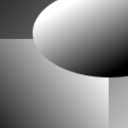
\includegraphics[width=\linewidth]{theme_cvpr/synth.png}
              \caption{Synthetic Image\\Size: 128 x 128\\grayscale\\\\}
            \endminipage\hfill
            \minipage{0.32\textwidth}
              
\includegraphics[width=\linewidth]{theme_cvpr/synthd.png}
              \caption{Boyle-Dysktra\\Level: 16\\Memory Used: 1.33 GB\\Runtime: 4505 s\\Iterations: 1000}
            \endminipage\hfill
            \minipage{0.32\textwidth}%
              
\includegraphics[width=\linewidth]{theme_cvpr/synthl.png}
              \caption{Lagrange-Multipliers\\Level: 16\\Memory Used: 0.155 GB\\Runtime: 10.39 s\\Iterations: 1000}
            \endminipage
        \end{figure}

    }

    \frame{
        \frametitle{Synthetic Image With Gaussian Noise (Size: 128 x 128)}

        \begin{figure}[!htb]
            \minipage{0.32\textwidth}
              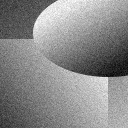
\includegraphics[width=\linewidth]{theme_cvpr/synthgauss.png}
              \caption{Noisy Image\\Size: 128 x 128\\grayscale\\\\}
            \endminipage\hfill
            \minipage{0.32\textwidth}
              
\includegraphics[width=\linewidth]{theme_cvpr/synthgaussd.png}
              \caption{Boyle-Dysktra\\Level: 16\\Memory Used: 1.33 GB\\Runtime: 4495 s\\Iterations: 1000}
            \endminipage\hfill
            \minipage{0.32\textwidth}%
              
\includegraphics[width=\linewidth]{theme_cvpr/synthgaussl.png}
              \caption{Lagrange-Multipliers\\Level: 16\\Memory Used: 0.155 GB\\Runtime: 10.47 s\\Iterations: 1000}
            \endminipage
        \end{figure}

    }

    \frame{
        \frametitle{La dama con l'ermellino (Size: 128 x 128)}

        \begin{figure}[!htb]
            \minipage{0.32\textwidth}
              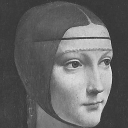
\includegraphics[width=\linewidth]{theme_cvpr/ladama.png}
              \caption{La dama Image\\Size: 128 x 128\\grayscale\\\\}
            \endminipage\hfill
            \minipage{0.32\textwidth}
              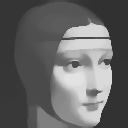
\includegraphics[width=\linewidth]{theme_cvpr/ladamad.png}
              \caption{Boyle-Dysktra\\Level: 16\\Memory Used: 1.33 GB\\Runtime: 4495 s\\Iterations: 1000}
            \endminipage\hfill
            \minipage{0.32\textwidth}%
              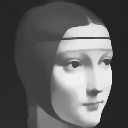
\includegraphics[width=\linewidth]{theme_cvpr/ladamal.png}
              \caption{Lagrange-Multipliers\\Level: 16\\Memory Used: 0.155 GB\\Runtime: 10.42 s\\Iterations: 1000}
            \endminipage
        \end{figure}

    }

    \frame{
        \frametitle{Crack Tip Inpainting (Size: 128 x 128)}

        \begin{figure}[!htb]
            \minipage{0.32\textwidth}
              
\includegraphics[width=\linewidth]{theme_cvpr/inpaint.png}
              \caption{Crack Tip Problem\\Size: 128 x 128\\grayscale\\\\}
            \endminipage\hfill
            \minipage{0.32\textwidth}
              
\includegraphics[width=\linewidth]{theme_cvpr/inpaintd.png}
              \caption{Boyle-Dysktra\\Level: 16\\Memory Used: 1.33 GB\\Runtime: 4501 s\\Iterations: 1000}
            \endminipage\hfill
            \minipage{0.32\textwidth}%
              
\includegraphics[width=\linewidth]{theme_cvpr/inpaintl.png}
              \caption{Lagrange-Multipliers\\Level: 16\\Memory Used: 0.155 GB\\Runtime: 10.49 s\\Iterations: 1000}
            \endminipage
        \end{figure}

    }

    \frame{
        \frametitle{Special Thanks To}

        \begin{itemize}
            \item Prof. Dr. Daniel Cremers
            \item Evgeny Strekalovskiy
            \item Thomas Moellenhoff
        \end{itemize}
    }

\frame[allowframebreaks]{
    \frametitle{Bibliography}
    \bibliography{bibliography}
    \begin{thebibliography}{56}
    \tiny

        \bibitem[iccv09]{iccv09}
        T. Pock and D. Cremers and H. Bischof and A. Chambolle,
        An Algorithm for Minimizing the Piecewise Smooth Mumford-Shah Functional,
        iccv,
        2009.
        \bibitem[pami11]{pami11}
        D. Cremers and K. Kolev
        Multiview Stereo and Silhouette Consistency via Convex Functionals over Convex Domains,
        pami,
        2011.

        
    \end{thebibliography}
    }

\end{document}
